% AI-GENERATED DEMONSTRATION — NOT PEER REVIEWED — NOT FOR CITATION
% agentic-research-examples: AI-generated demonstration for the tutorial "Easing into agentic AI in research". See AI_GENERATED.md.
% Options for packages loaded elsewhere
\PassOptionsToPackage{unicode}{hyperref}
\PassOptionsToPackage{hyphens}{url}
\PassOptionsToPackage{dvipsnames,svgnames,x11names}{xcolor}
\documentclass[
  british,
  11pt,
]{article}
\usepackage{xcolor}
\usepackage[margin=1in]{geometry}
\usepackage{amsmath,amssymb}
\setcounter{secnumdepth}{-\maxdimen} % remove section numbering
\usepackage{iftex}
\ifPDFTeX
  \usepackage[T1]{fontenc}
  \usepackage[utf8]{inputenc}
  \usepackage{textcomp} % provide euro and other symbols
\else % if luatex or xetex
  \usepackage{unicode-math} % this also loads fontspec
  \defaultfontfeatures{Scale=MatchLowercase}
  \defaultfontfeatures[\rmfamily]{Ligatures=TeX,Scale=1}
\fi
\usepackage{lmodern}
\ifPDFTeX\else
  % xetex/luatex font selection
\fi
% Use upquote if available, for straight quotes in verbatim environments
\IfFileExists{upquote.sty}{\usepackage{upquote}}{}
\IfFileExists{microtype.sty}{% use microtype if available
  \usepackage[]{microtype}
  \UseMicrotypeSet[protrusion]{basicmath} % disable protrusion for tt fonts
}{}
\usepackage{setspace}
\makeatletter
\@ifundefined{KOMAClassName}{% if non-KOMA class
  \IfFileExists{parskip.sty}{%
    \usepackage{parskip}
  }{% else
    \setlength{\parindent}{0pt}
    \setlength{\parskip}{6pt plus 2pt minus 1pt}}
}{% if KOMA class
  \KOMAoptions{parskip=half}}
\makeatother
\usepackage{longtable,booktabs,array}
\newcounter{none} % for unnumbered tables
\usepackage{calc} % for calculating minipage widths
% Correct order of tables after \paragraph or \subparagraph
\usepackage{etoolbox}
\makeatletter
\patchcmd\longtable{\par}{\if@noskipsec\mbox{}\fi\par}{}{}
\makeatother
% Allow footnotes in longtable head/foot
\IfFileExists{footnotehyper.sty}{\usepackage{footnotehyper}}{\usepackage{footnote}}
\makesavenoteenv{longtable}
\usepackage{graphicx}
\makeatletter
\newsavebox\pandoc@box
\newcommand*\pandocbounded[1]{% scales image to fit in text height/width
  \sbox\pandoc@box{#1}%
  \Gscale@div\@tempa{\textheight}{\dimexpr\ht\pandoc@box+\dp\pandoc@box\relax}%
  \Gscale@div\@tempb{\linewidth}{\wd\pandoc@box}%
  \ifdim\@tempb\p@<\@tempa\p@\let\@tempa\@tempb\fi% select the smaller of both
  \ifdim\@tempa\p@<\p@\scalebox{\@tempa}{\usebox\pandoc@box}%
  \else\usebox{\pandoc@box}%
  \fi%
}
% Set default figure placement to htbp
\def\fps@figure{htbp}
\makeatother
% definitions for citeproc citations
\NewDocumentCommand\citeproctext{}{}
\NewDocumentCommand\citeproc{mm}{%
  \begingroup\def\citeproctext{#2}\cite{#1}\endgroup}
\makeatletter
 % allow citations to break across lines
 \let\@cite@ofmt\@firstofone
 % avoid brackets around text for \cite:
 \def\@biblabel#1{}
 \def\@cite#1#2{{#1\if@tempswa , #2\fi}}
\makeatother
\newlength{\cslhangindent}
\setlength{\cslhangindent}{1.5em}
\newlength{\csllabelwidth}
\setlength{\csllabelwidth}{3em}
\newenvironment{CSLReferences}[2] % #1 hanging-indent, #2 entry-spacing
 {\begin{list}{}{%
  \setlength{\itemindent}{0pt}
  \setlength{\leftmargin}{0pt}
  \setlength{\parsep}{0pt}
  % turn on hanging indent if param 1 is 1
  \ifodd #1
   \setlength{\leftmargin}{\cslhangindent}
   \setlength{\itemindent}{-1\cslhangindent}
  \fi
  % set entry spacing
  \setlength{\itemsep}{#2\baselineskip}}}
 {\end{list}}
\usepackage{calc}
\newcommand{\CSLBlock}[1]{\hfill\break\parbox[t]{\linewidth}{\strut\ignorespaces#1\strut}}
\newcommand{\CSLLeftMargin}[1]{\parbox[t]{\csllabelwidth}{\strut#1\strut}}
\newcommand{\CSLRightInline}[1]{\parbox[t]{\linewidth - \csllabelwidth}{\strut#1\strut}}
\newcommand{\CSLIndent}[1]{\hspace{\cslhangindent}#1}
\ifLuaTeX
\usepackage[bidi=basic,shorthands=off]{babel}
\else
\usepackage[bidi=default,shorthands=off]{babel}
\fi
\ifLuaTeX
  \usepackage{selnolig} % disable illegal ligatures
\fi
\setlength{\emergencystretch}{3em} % prevent overfull lines
\providecommand{\tightlist}{%
  \setlength{\itemsep}{0pt}\setlength{\parskip}{0pt}}
\usepackage{needspace}
\usepackage{etoolbox}
\AtBeginEnvironment{CSLReferences}{\interlinepenalty=10000}
\widowpenalty=10000
\clubpenalty=10000
\usepackage{float}
\floatplacement{figure}{H}
\usepackage{bookmark}
\IfFileExists{xurl.sty}{\usepackage{xurl}}{} % add URL line breaks if available
\urlstyle{same}
% fallback for those not using the hyperref driver hyperxmp:
\makeatletter
\@ifundefined{xmpquote}{\newcommand{\xmpquote}[1]{#1}}{}
\makeatother
\hypersetup{
  pdftitle={Learning from disagreements: When selective feedback helps and harms advisor evaluation},
  pdfauthor={Lukas Wallrich --- draft; author approval pending},
  pdflang={en-GB},
  colorlinks=true,
  linkcolor={Maroon},
  filecolor={Maroon},
  citecolor={Blue},
  urlcolor={Blue},
  pdfcreator={LaTeX via pandoc}}

\title{Learning from disagreements: When selective feedback helps and
harms advisor evaluation}
\author{Lukas Wallrich --- draft; author approval pending}
\date{}

\begin{document}
\maketitle

\setstretch{1.15}
\section{Abstract}\label{abstract}

Outcome feedback can be accurate about the cases it reveals yet
misleading about an advisor's overall competence. I distinguish
estimating absolute advisor accuracy from deciding whether the advisor
is more accurate than oneself. Uniformly sampled disagreements preserve
the sign of the paired accuracy difference, although comparing the
advisor's selected accuracy with one's marginal accuracy can reject a
superior advisor. Confidence-dependent verification can remove this
protection. A prospectively specified simulation compared absolute,
paired, inverse-probability-weighted, and capped-weight summaries at
fixed feedback budgets. In the prespecified crossing-advantage scenario,
weighting reduced deployment regret by 4.357 percentage points (97.5\%
Monte Carlo interval {[}-4.383, -4.332{]} for weighted minus paired
regret). In a control with the same marginal source accuracies but a
positive advisor advantage in both confidence strata, weighting
increased regret by 1.112 points at the smaller budget and stronger
selection ratio; the directions also held at matched budgets and ratios.
These model consequences show that correcting selection can help or harm
a finite-feedback decision within a global adoption task. The model
generates a refutable prediction for an experiment crossing feedback
selection with the display of absolute or paired accuracy. Its
behavioural interpretation remains untested: simulated decision makers
implement stipulated estimators, and the study does not demonstrate how
people learn from selective feedback.

\textbf{Keywords:} advice taking; selective feedback; confidence;
comparative accuracy; simulation; inverse probability weighting

\section{Introduction}\label{introduction}

A person who verifies an advisor's recommendation learns whether that
recommendation was correct. Across cases, however, verified
recommendations need not represent the advice the person will receive
next. Disagreements may be especially likely to attract scrutiny, and
people may preferentially check disagreements when they feel confident
in their own answer. The resulting feedback can answer a different
question from the one used to decide whether to adopt the advisor. This
paper asks when feedback that is selective in this way still supports a
sound comparative judgement, and when correcting its selection improves
the eventual decision.

The distinction matters because the practical question is often
comparative. A person deciding whether to use an advisor may need to
know whether its decisions are better than their own, without needing an
unbiased estimate of either source's absolute accuracy. Conversely, an
apparently low advisor hit rate need not justify rejecting it if one's
own hit rate on those same cases is lower. I analyse this distinction in
a deliberately constrained setting: after observing verified cases, a
decision maker selects either their own initial judgements or the
advisor for a new, randomly drawn set of cases. The model concerns this
global adoption decision; it does not optimise which source to use on
each individual case.

\subsection{What feedback makes
available}\label{what-feedback-makes-available}

Research on advice taking already distinguishes agreement from accuracy.
Pescetelli and Yeung (2021) showed how decision confidence contributes
to advice taking and trust formation, including how agreement and
confidence can supply evidence when objective feedback is unavailable.
Their account also exposes distortions when judgements are dependent.
Jaquiery and Yeung (2024) experimentally separated preferences for
agreement and accuracy; objective feedback supported a preference for
accurate advice. These findings motivate attention to the evidence on
which advisor judgements rest, but they do not establish how people
interpret feedback selected from disagreements.

Learning depends on which outcomes can be observed and how feedback is
interpreted (Einhorn \& Hogarth, 1978). Selective experience can sustain
inaccurate impressions without requiring intrinsically hostile
attitudes. Denrell and March (2001) formalised how adaptive choices
restrict later information, and Denrell (2005) applied experience
sampling to impression formation. In interpersonal trust, Fetchenhauer
and Dunning (2010) found that feedback supplied independently of the
decision to trust reduced excessive scepticism. These studies establish
the broader sampling problem. They do not imply that every comparative
inference requires representative feedback: uniformly sampled
disagreements can identify the comparative sign because the excluded
agreements contribute zero to the difference. Unverified disagreements
do not have zero contributions; their selection must still be accounted
for.

Selective feedback need not produce naive inference. Elwin et al. (2007)
found that a constructivist account of how people encoded observed and
missing feedback described their tasks better than simply learning from
observed outcomes. Their design also approximately matched the amount of
feedback across selection conditions by allowing more opportunities
under selective feedback. The present paper therefore treats naive
summaries as candidate rules, not an established description of people.

Verification and learning from verified cases are also distinct. Fok and
Weld (2024) argue that explanations help human--AI decision making when
they enable verification. Honeycutt et al. (2020) found that soliciting
interactive feedback could reduce users' trust and impressions of model
accuracy. Neither result implies the mechanism modelled here. The
present analysis assumes that verification accurately reveals the truth
and asks what can then be inferred from the selected history. It
therefore concerns a downstream problem even when verification itself
succeeds.

Recent computational work further limits the claim to priority. Gao et
al. (2021) used inverse-probability weighting in learning human--AI
routing from bandit feedback. Their problem involves selectively
observed rewards and policies that exploit complementary performance.
Zavattari et al. (2026), in a recent preprint, analyse allocation of a
human audit budget across an agent fleet, including confidence
dependence and updating after audits. Li and Steyvers (2026), also in a
preprint, examine learning the relationship between AI confidence and
accuracy. The contribution here is neither weighting nor learning
advisor reliability in general. It is the comparison of absolute and
paired feedback summaries for a global adoption decision, together with
the finite-feedback consequences of correcting selection within
disagreements.

\subsection{The present study}\label{the-present-study}

I first establish which comparative conclusions follow directly from the
sampling mechanism. These are analytic properties rather than simulated
discoveries. I then compare the decision losses induced by several
summaries when only a finite set of verified outcomes is available. The
registered computational predictions anticipate a benefit of weighting
when confidence selection reverses the population comparison and a cost
when selection instead favours informative comparisons. Finally, I
specify a feedback-display experiment that could reject the proposed
connection between these summaries and human judgement. No human outcome
data are analysed, and no behavioural mechanism is considered confirmed
by the simulation.

\section{Analytic framework}\label{analytic-framework}

Consider a two-alternative decision with exactly one correct response.
Let \(A\) and \(H\) indicate the correctness of the advisor's and
human's initial responses; disagreements therefore imply \(A+H=1\). Let
\(D\) indicate disagreement between those responses, \(d=P(D)\),
\(h=E[H]\), and \(\Delta=E[A-H]\). On an agreement, \(A-H=0\).
Therefore, for \(d>0\),

\[E[A-H\mid D]=\frac{\Delta}{d}.\]

Uniform disagreement feedback preserves the sign of the overall accuracy
advantage. It does not recover its magnitude without \(d\), nor does it
identify either marginal accuracy. This connects to the classical
comparison of correlated proportions (McNemar, 1947); here the identity
follows directly from the zero contribution of agreements. On a binary
disagreement exactly one source is correct, so

\[E[A\mid D]=\frac{1+\Delta/d}{2}.\]

An absolute summary compared with the known marginal human benchmark
favours the advisor only when \(\Delta>d(2h-1)\). A paired summary
instead favours it whenever \(\Delta>0\). This comparison isolates an
estimand mismatch: both the numerator and the benchmark must refer to
the same selected cases. It is not a general claim that selected advisor
accuracy must be biased downward.

Now distinguish low- and high-confidence strata with population
proportions \(p\) and \(1-p\), and within-stratum marginal advisor
advantages \(\delta_c=E[A-H\mid C=c]\), for \(c=L,H\). These contrasts
include both agreements and disagreements within each stratum. Within
each confidence stratum, verification is random among disagreements. Let
\(k=\pi_H/\pi_L\ge1\) be the ratio of high- to low-confidence
verification probabilities among disagreements. The sign of the selected
paired comparison is then the sign of

\[p\delta_L+(1-p)k\delta_H.\]

Let \(d_c=P(D\mid C=c)\). The audited numerator contains
\(p d_L E[A-H\mid D,L]+(1-p)k d_H E[A-H\mid D,H]\); substituting
\(d_cE[A-H\mid D,c]=\delta_c\) gives the preceding expression. Selection
can reverse the global ordering when conditional advantages have
opposite signs. If the advisor is better in both strata, positive
reweighting cannot reverse the population sign. Inverse selection
weights recover the sign of \(\Delta\), provided both disagreement
strata have positive sampling probability and verification is
independent of which source is correct within each stratum. With sample
normalisation, the resulting score estimates the mean contrast among all
disagreements, \(\Delta/d\), rather than the unscaled global advantage.
A capped weight generally targets a different selected contrast. Neither
the unweighted nor the normalised weighted estimate is treated as a
universally unbiased estimate of global accuracy difference.

For \(\delta_L>0>\delta_H\), the sign changes at
\(k^*=p\delta_L/[(1-p)|\delta_H|]\). If the true ratio is \(k\) but the
low-stratum weight is \(w\), the corrected numerator is proportional to
\(p\delta_L w/k+(1-p)\delta_H\). Capping substitutes \(w=\min(k,b)\) for
cap \(b\). These expressions also describe misspecified weights. The
sign suffices only for a cost-free choice between sources: a non-zero
adoption cost requires the magnitude \(\Delta\), and therefore the
disagreement rate as well as its conditional contrast. The disagreement
rate itself is observable without truth labels when both initial
responses are recorded.

Finite samples make the policy comparison less straightforward. Weights
amplify contributions from rarely verified cases, potentially increasing
decision error even when their limiting target is appropriate. Moreover,
correcting a harmless selection can discard its informational advantage.
The simulation quantifies these losses under explicit environments and
feedback budgets. It does not require simulation to establish the
preceding identities.

\subsection{Exact finite-feedback
risk}\label{exact-finite-feedback-risk}

The finite-label comparisons can be calculated without Monte Carlo
approximation. Let \(Q_j\) be the probability of audited category \(j\)
and let \(u_{mj}\) be its contribution to summary \(m\) before a
positive normalising denominator: \(A-h\) for absolute evaluation,
\(A-H\) for pairing, and \(w(C)(A-H)\) for weighted pairing. For
rational scenario parameters, choose a positive common denominator \(M\)
and define integer increments \(\tilde u_{mj}=M u_{mj}\). This rescaling
preserves zero scores and the sign of every score. Define the finite
Laurent polynomial

\[G_m(z)=\sum_j Q_j z^{\tilde u_{mj}}.\]

After \(n\) independent labels, \(P(\tilde S_m=s)=[z^s]G_m(z)^n\). For
\(\Delta\ne0\), expected regret is therefore

\[R_m(n)=|\Delta|\left\{\sum_{s:\,s\Delta<0}[z^s]G_m(z)^n+\tfrac12[z^0]G_m(z)^n\right\}.\]

Here \([z^0]G_m(z)^n\) is the exact score-tie probability, and its half
weight implements fair random choice. For a marginal accuracy tie regret
is zero. The finite-budget boundary between two summaries is
\(R_m(n)=R_{m'}(n)\), evaluated by convolution of these score
distributions. An analyst knowing the scenario probabilities can compute
this boundary; the simulated learner receives the sampled cases and its
specified benchmark or weights, not the true risk. This formula explains
the exact checks and supports the exploratory matched-pattern analysis.
For a fixed number of encountered cases, the same convolution instead
uses encounter-category probabilities, including an unaudited category
with zero score. Simulation provides a separately implemented numerical
check and preserves the prospectively specified analysis.

\section{Method}\label{method}

\subsection{Prospective specification and
reproducibility}\label{prospective-specification-and-reproducibility}

The hypotheses, environments, estimators, exclusions, and inference
criteria were committed locally before hypothesis-bearing computation
(git commit \texttt{68c07e4}). This provides a recoverable prospective
record, not an independently timestamped public registration. Before
that commitment, the workflow examined published articles, dataset
documentation, and idea reviews, but no participant-level outcomes or
hypothesis simulations. No existing dataset was used. A previous project
remained in repository history; its deleted outcomes and manuscripts
were not inspected.

The command \texttt{./run\_all.sh} regenerates synthetic raw count
histories, analyses, numerical checks, figures, and the manuscript.
Saved count histories are sufficient for every estimator because
feedback order is not used. Configuration, seeds, software versions, and
hashes accompany the results. The main specification was followed;
implementation clarifications and any later reviewer-requested analyses
are documented in \texttt{deviations.md}. Full decisions, source audits,
deviations, and reviewer responses accompany the manuscript. OpenAI
Codex generated the study design and analysis code, executed the
scripts, and checked results with a separate implementation; all
reported results come from these scripts. The Transparency and
declarations section and \texttt{ai\_disclosure.md} identify the tools,
review models, dates, access routes, and scope of assistance.

\subsection{Environments and
selection}\label{environments-and-selection}

Human correctness probabilities were 0.60 and 0.90 in low- and
high-confidence strata. These are calibrated confidence categories by
construction, not estimates from human ratings. The grid crossed
low-confidence shares 0.25, 0.50, 0.75, advisor low-confidence
accuracies 0.65, 0.80, 0.95, advisor high-confidence accuracies 0.70,
0.80, 0.90, and overlap positions 0.00, 0.50, 1.00, yielding 81
environments. An additional homogeneous-advantage control brought the
total to 82. Every registered grid environment has
\(\delta_L>0\ge\delta_H\). High-confidence oversampling therefore shifts
the paired comparison towards the human: it can reverse a superior
advisor's ranking but reinforces the correct ranking of an inferior
advisor. Results for other sign patterns come only from the later
exploratory extension, whose conditional advantage magnitudes are
deliberately narrow.

For each stratum with marginal accuracies \(h_c,a_c\), the probability
of both sources being correct was

\[q_c=\max(0,h_c+a_c-1)+r\{\min(h_c,a_c)-\max(0,h_c+a_c-1)\}.\]

The four joint masses were \(q_c,h_c-q_c,a_c-q_c,1-h_c-a_c+q_c\). Thus
the dependence parameter \(r\) locates the joint distribution within its
feasible bounds; it is not a correlation coefficient. For binary
decisions, disagreement is equivalent to exactly one response being
correct. The model uses only this relation and the joint correctness
probabilities; no truth-prevalence estimate or perceptual mechanism is
needed. At feasible-bound endpoints, some outcome categories have zero
probability. Those boundary cases remain in the grid and can make some
comparisons deterministic.

The focal crossing environment used equal stratum shares, midpoint
overlap, and advisor accuracy 0.80 in both strata. The advisor was
better at low confidence and worse at high confidence, while its
marginal accuracy was 0.80 against human accuracy 0.75. The homogeneous
control had advisor accuracies 0.65 and 0.95, retaining the same
marginal accuracies but a positive advantage in both strata. These
scenarios were selected in advance to contrast two mechanisms; they are
not empirical prevalence estimates. Their conditional advantages were
chosen deliberately to cross or remain positive, with the analytic
selection boundary in view. They also differ in disagreement rate and
conditional informativeness; the focal contrasts further use different
budgets and ratios. Thus the two predictions illustrate contrasting
conditions rather than isolate a single causal factor. Matched
comparisons are also reported.

Feedback was either a random sample of all cases or a sample of
disagreements with high-to-low verification ratios 1, 2, 4, 8. Under
disagreement schedules, verification probabilities were \(1/k\) at low
confidence and unity at high confidence; agreements were never verified.
Histories contained 20, 100, 500 independent verified outcomes. Matching
verified outcomes holds the feedback budget constant but does not equate
the number of cases encountered. I therefore also report audit yield and
the expected opportunities needed to obtain each history.

\subsection{Summaries and adoption
rule}\label{summaries-and-adoption-rule}

The absolute learner subtracted known marginal human accuracy from
observed advisor accuracy. The paired learner averaged \(A-H\) on
verified cases. The inverse-probability-weighted learner averaged the
same difference using weights \(k\) and unity in the low- and
high-confidence disagreement strata, divided by their realised total.
The capped learner limited these weights to 2, a prospectively fixed,
intentionally simple intermediate correction. Under random feedback all
weights were equal.

Each learner selected the advisor for a positive score and the human for
a negative score. A numerical tie within 1e-12 was averaged over fair
random selection. Learners within a condition used identical histories,
permitting paired Monte Carlo contrasts. The known human benchmark gives
the absolute learner information beyond the observed sample; it is a
deliberate, favourable-information assumption. Every rule was computed
from the same paired records; the absolute rule uses only the advisor
component. The paired rules use both components, and the implemented
weighting rule additionally receives confidence-stratum labels and the
true sampling ratio. Calibration makes the strata psychologically
interpretable but is not required for the weighting algebra.

Known ratios are sufficient, not necessary, for a feasible correction.
If both initial responses and confidence are recorded on all encountered
cases, their unlabelled disagreements identify the population stratum
masses \(p_c d_c\). Verification counts can estimate the selection
ratio. Alternatively, post-stratification estimates
\(\widehat\Delta=\sum_c \widehat{p_c d_c}\,\overline{(A-H)}_{V,D,c}\),
where the final factor is the mean among verified disagreements in
stratum \(c\). Under conditional random verification and positive
support, this estimator is consistent without a disclosed ratio. Empty
verified strata require an additional finite-sample rule, such as a
preregistered prior on their contrast or retaining the baseline until
each stratum has feedback. Such choices add assumptions or change the
stopping policy and must be evaluated in their own right. These
encounter-level estimators are not evaluated here: estimating masses or
weights changes sampling variability and dependence, so neither their
finite-sample risk nor the direction of every known-weight contrast
follows from this study. The misspecified-weight analysis concerns a
rule using an externally supplied or assumed ratio; observed encounter
counts could help prevent that error.

The outcome was expected deployment regret: the accuracy loss on a
future random case relative to the better fixed source. It equals
\(|\Delta|\) multiplied by the probability of selecting the inferior
source. This benchmark cannot establish complementary team performance
and does not exploit confidence-contingent delegation. When marginal
accuracies tie, regret is zero and ranking error is undefined; those
environments remain in the output.

\subsection{Registered predictions and numerical
precision}\label{registered-predictions-and-numerical-precision}

\textbf{H1:} In the crossing environment with verification ratio 4 and
100 verified outcomes, weighted paired evaluation produces less regret
than unweighted paired evaluation.

\textbf{H2:} In the homogeneous control with verification ratio 8 and 20
verified outcomes, weighted paired evaluation produces more regret than
unweighted paired evaluation.

Each condition contained 20,000 independent histories generated with
NumPy PCG64 and seed 20260928. Separate child streams were assigned to
conditions in fixed order. For each hypothesis, I estimated weighted
minus paired regret within the same histories and calculated a 97.5\%
normal Monte Carlo interval. The prespecified Bonferroni adjustment
covers the 2 contrasts jointly at approximately 95\%. A wholly
predicted-side interval supports the computational prediction; a wholly
opposite-side interval contradicts it; overlap with zero is unresolved.
These intervals describe numerical integration precision. The outcomes
are fixed consequences of the stipulated model, and prospective
specification constrains the reporting choices rather than creating
empirical uncertainty. An independently implemented exact convolution
subsequently evaluated the focal score distributions; those calculations
verify the simulated contrasts. The output retains the original support
labels to preserve the registered decision rule, while the text reports
the numerical directions.

All scenarios, budgets, and learners were retained. Additional
prespecified descriptions included adoption probabilities, limiting
scores, capped correction, audit yields, and the lowest tested budget at
which weighting improved estimated regret. Grid comparisons used the
prespecified regret tolerance 0.0005 in proportion units (0.05
percentage points); they are descriptions of a chosen design, not
statistical generalisations to a population of tasks.

\section{Results}\label{results}

\subsection{Registered numerical
comparisons}\label{registered-numerical-comparisons}

Both registered contrasts had the predicted direction. Independent exact
values fell inside their Monte Carlo intervals (Table 1).

{\def\LTcaptype{none} % do not increment counter
\begin{longtable}[]{@{}
  >{\raggedright\arraybackslash}p{(\linewidth - 8\tabcolsep) * \real{0.2000}}
  >{\raggedleft\arraybackslash}p{(\linewidth - 8\tabcolsep) * \real{0.2000}}
  >{\raggedleft\arraybackslash}p{(\linewidth - 8\tabcolsep) * \real{0.2000}}
  >{\raggedright\arraybackslash}p{(\linewidth - 8\tabcolsep) * \real{0.2000}}
  >{\raggedright\arraybackslash}p{(\linewidth - 8\tabcolsep) * \real{0.2000}}@{}}
\toprule\noalign{}
\begin{minipage}[b]{\linewidth}\raggedright
Prediction
\end{minipage} & \begin{minipage}[b]{\linewidth}\raggedleft
Monte Carlo difference
\end{minipage} & \begin{minipage}[b]{\linewidth}\raggedleft
Exact difference
\end{minipage} & \begin{minipage}[b]{\linewidth}\raggedright
Monte Carlo interval
\end{minipage} & \begin{minipage}[b]{\linewidth}\raggedright
Direction
\end{minipage} \\
\midrule\noalign{}
\endhead
\bottomrule\noalign{}
\endlastfoot
H1 & -4.357 & -4.344 & {[}-4.383, -4.332{]} & weighted lower \\
H2 & 1.112 & 1.088 & {[}1.079, 1.145{]} & weighted higher \\
\end{longtable}
}

\emph{Table 1. Prespecified regret contrasts with independent exact
checks. Regret and contrasts are percentage points of expected accuracy
on a future random case. Intervals quantify Monte Carlo uncertainty,
with the family-wise adjustment specified before computation.}

\subsection{What the selected cases
imply}\label{what-the-selected-cases-imply}

In the crossing environment, uniform disagreement feedback gave the
advisor a limiting selected accuracy of 58.333\%, against the known
marginal human benchmark of 75.0\%. The paired contrast was positive at
0.167, correctly favouring the advisor. With high-confidence
verification ratio 4, the selected advisor accuracy became 41.667\% and
the paired contrast became -0.167. Weighting restored the limiting
contrast to 0.167. The crossing environment has reversal threshold 2. At
that ratio the limiting paired contrast is zero; at ratio 4, the
registered cap also produces a zero limiting contrast. Capped adoption
near chance in this scenario reflects this neutral boundary. Under
random feedback, the absolute rule benefits from its supplied true human
benchmark and avoids estimating human accuracy from the feedback sample.

\Needspace{27\baselineskip}

{\def\LTcaptype{none} % do not increment counter
\begin{longtable}[]{@{}
  >{\raggedright\arraybackslash}p{(\linewidth - 12\tabcolsep) * \real{0.1429}}
  >{\raggedright\arraybackslash}p{(\linewidth - 12\tabcolsep) * \real{0.1429}}
  >{\raggedleft\arraybackslash}p{(\linewidth - 12\tabcolsep) * \real{0.1429}}
  >{\raggedleft\arraybackslash}p{(\linewidth - 12\tabcolsep) * \real{0.1429}}
  >{\raggedleft\arraybackslash}p{(\linewidth - 12\tabcolsep) * \real{0.1429}}
  >{\raggedleft\arraybackslash}p{(\linewidth - 12\tabcolsep) * \real{0.1429}}
  >{\raggedleft\arraybackslash}p{(\linewidth - 12\tabcolsep) * \real{0.1429}}@{}}
\toprule\noalign{}
\begin{minipage}[b]{\linewidth}\raggedright
Environment
\end{minipage} & \begin{minipage}[b]{\linewidth}\raggedright
Selection
\end{minipage} & \begin{minipage}[b]{\linewidth}\raggedleft
Labels
\end{minipage} & \begin{minipage}[b]{\linewidth}\raggedleft
Absolute
\end{minipage} & \begin{minipage}[b]{\linewidth}\raggedleft
Paired
\end{minipage} & \begin{minipage}[b]{\linewidth}\raggedleft
Weighted
\end{minipage} & \begin{minipage}[b]{\linewidth}\raggedleft
Capped
\end{minipage} \\
\midrule\noalign{}
\endhead
\bottomrule\noalign{}
\endlastfoot
crossing & all cases & 100 & 88.9\% & 81.9\% & 81.9\% & 81.9\% \\
crossing & disagreements, k = 1 & 100 & 0.0\% & 95.4\% & 95.4\% &
95.4\% \\
crossing & disagreements, k = 4 & 100 & 0.0\% & 4.7\% & 91.9\% &
49.2\% \\
crossing & disagreements, k = 4 & 500 & 0.0\% & 0.0\% & 99.9\% &
49.9\% \\
homogeneous & disagreements, k = 8 & 20 & 27.9\% & 95.6\% & 73.3\% &
91.0\% \\
homogeneous & disagreements, k = 8 & 100 & 8.7\% & 100.0\% & 92.4\% &
99.9\% \\
homogeneous & disagreements, k = 8 & 500 & 0.1\% & 100.0\% & 100.0\% &
100.0\% \\
\end{longtable}
}

\emph{Table 2. Advisor adoption probabilities in focal environments.
Each row uses the same histories across summaries; selection refers to
the high-to-low verification ratio among disagreements. The advisor is
globally superior in both environments. Adoption is the proportion of
histories choosing it, counting a tied history as half an adoption.
Entries come from the prespecified simulation, including the
random-feedback benchmark. The machine-readable output retains unrounded
probabilities and tie rates.}

\begin{figure}
\centering
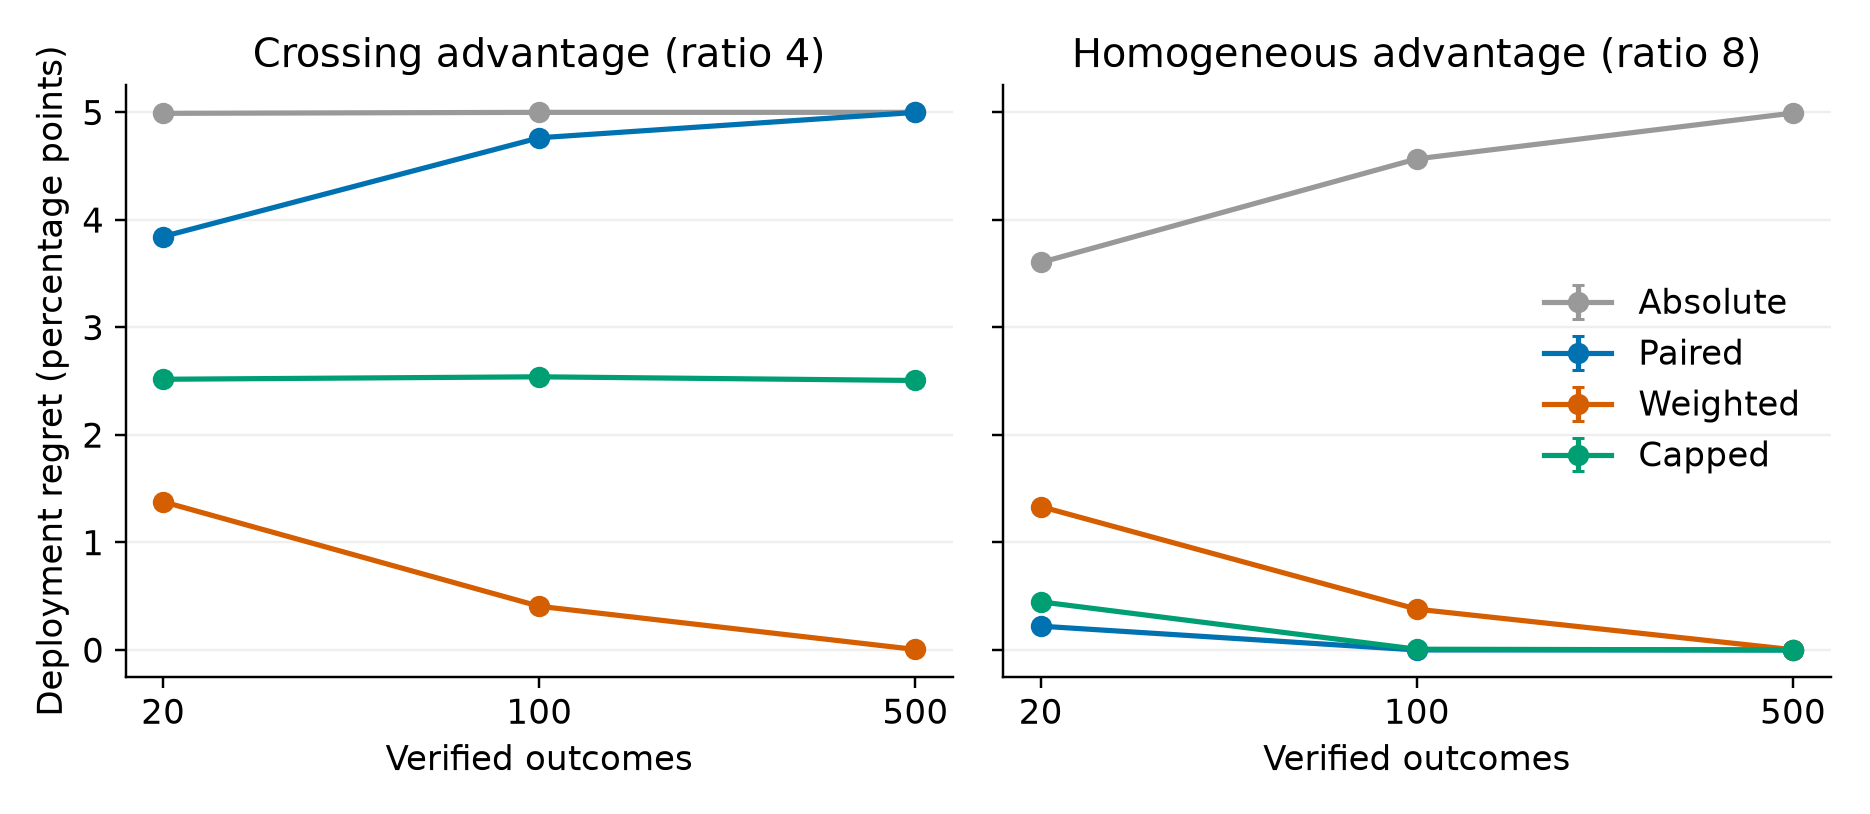
\includegraphics[width=1\linewidth,height=\textheight,keepaspectratio,alt={Expected deployment regret by feedback budget and summary in the focal environments. Error bars show Monte Carlo intervals at the registered level and may be smaller than the markers. Points are prespecified budgets; lines guide the eye and do not estimate intermediate budgets. Errors concern global source adoption.}]{figures/focal_regret.png}
\caption{Expected deployment regret by feedback budget and summary in
the focal environments. Error bars show Monte Carlo intervals at the
registered level and may be smaller than the markers. Points are
prespecified budgets; lines guide the eye and do not estimate
intermediate budgets. Errors concern global source adoption.}
\end{figure}

\subsection{Prespecified grid and resource
descriptions}\label{prespecified-grid-and-resource-descriptions}

The registered grid included 54 superior-advisor environments, 24
inferior-advisor environments, and 3 exact marginal ties. All have a
positive low-confidence and nonpositive high-confidence advisor
advantage. At ratio 8, the limiting paired sign reversed the global
ordering in 24 environments, all with globally superior advisors.

\Needspace{17\baselineskip}

{\def\LTcaptype{none} % do not increment counter
\begin{longtable}[]{@{}
  >{\raggedright\arraybackslash}p{(\linewidth - 8\tabcolsep) * \real{0.2000}}
  >{\raggedleft\arraybackslash}p{(\linewidth - 8\tabcolsep) * \real{0.2000}}
  >{\raggedleft\arraybackslash}p{(\linewidth - 8\tabcolsep) * \real{0.2000}}
  >{\raggedleft\arraybackslash}p{(\linewidth - 8\tabcolsep) * \real{0.2000}}
  >{\raggedleft\arraybackslash}p{(\linewidth - 8\tabcolsep) * \real{0.2000}}@{}}
\toprule\noalign{}
\begin{minipage}[b]{\linewidth}\raggedright
Advisor group
\end{minipage} & \begin{minipage}[b]{\linewidth}\raggedleft
Labels
\end{minipage} & \begin{minipage}[b]{\linewidth}\raggedleft
Lower regret
\end{minipage} & \begin{minipage}[b]{\linewidth}\raggedleft
Higher regret
\end{minipage} & \begin{minipage}[b]{\linewidth}\raggedleft
Within tolerance
\end{minipage} \\
\midrule\noalign{}
\endhead
\bottomrule\noalign{}
\endlastfoot
All & 20 & 44 & 22 & 15 \\
All & 500 & 36 & 9 & 36 \\
Superior & 500 & 36 & 0 & 18 \\
Inferior & 500 & 0 & 9 & 15 \\
Tied & 500 & 0 & 0 & 3 \\
\end{longtable}
}

\emph{Table 3. Registered environment counts comparing weighted with
paired regret at selection ratio 8. Subgroup rows partition the
all-environment row at the largest registered budget; this is a
finite-budget description, not an asymptotic result.}

Complete results, including all capped and dependence settings, are in
the machine-readable tables. Among inferior advisors, high-confidence
selection supports the correct ranking; correction removes some of that
support and can increase finite-label loss. No grid frequency estimates
the prevalence of such environments in practice. Categories use weighted
minus paired regret: below -0.0005, within the inclusive bounds ±0.0005,
or above 0.0005 in proportion units.

In the crossing scenario, uniform disagreement selection verified 30.0\%
of encountered cases, requiring an expected 333.3 opportunities for 100
labels. Selection ratio 4 reduced yield to 15.0\%, requiring 666.7
opportunities for the same label budget. In the homogeneous control,
ratio 8 required 266.7 expected opportunities for 20 labels. Random
all-case verification requires one opportunity per label. These are
expected acquisition costs under independent cases, not realised waiting
times.

Numerical checks verified the joint probability tables and margins,
analytic sign properties, equivalent learners under uniform weighting,
and exact binomial benchmarks for the focal uniform-disagreement
conditions. The saved verification report records each comparison and
its prespecified Monte Carlo tolerance. No history was excluded.
Independent exact convolution checked all 120 focal learner conditions.
The supplementary focal tie-probability table records ties explicitly;
fair random tie-breaking is integrated into every risk.

\subsection{Exploratory analyses}\label{exploratory-analyses}

The following analyses were added after seeing the registered results
and are exploratory. Exact discrete score convolutions compare fixed
encounter budgets and misspecified positive selection weights.

With 100 encountered cases in the crossing environment at ratio 4, the
expected label count was 15.0. Weighted and paired regret were 1.521 and
3.700 percentage points respectively (difference -2.179).

With 20 encountered cases in the homogeneous environment at ratio 8, the
expected label count was 1.5. Weighted and paired regret were 1.830 and
1.681 percentage points respectively (difference 0.149).

The contrast directions persisted at these encounter budgets, with
smaller magnitudes. At fixed encounters, random all-case verification
means verifying every encountered case. It has identical paired-rule
risk to uniform-disagreement verification: removing agreement labels
removes zero score contributions. Their label costs differ.

In the crossing environment, the limiting weighted ranking is correct
only when the assumed low-stratum weight exceeds half the true selection
ratio. Exact inverse weights need not minimise finite-feedback
classification loss: an incorrect weight can emphasise a favourable
stratum and improve one selected scenario while changing the target.
This prevents interpreting the weighting rule as a universally optimal
adoption policy.

For the crossing focal setting (true ratio 4, 100 labels), assumed
low-stratum weights 1, 2, 4, 8, 16 produced exact regret of 4.765,
2.512, 0.421, 0.070, 0.022 percentage points, respectively.

For the homogeneous focal setting (true ratio 8, 20 labels), assumed
low-stratum weights 1, 2, 4, 8, 16 produced exact regret of 0.214,
0.442, 0.877, 1.302, 1.525 percentage points, respectively.

{\def\LTcaptype{none} % do not increment counter
\begin{longtable}[]{@{}
  >{\raggedright\arraybackslash}p{(\linewidth - 10\tabcolsep) * \real{0.1667}}
  >{\raggedleft\arraybackslash}p{(\linewidth - 10\tabcolsep) * \real{0.1667}}
  >{\raggedleft\arraybackslash}p{(\linewidth - 10\tabcolsep) * \real{0.1667}}
  >{\raggedleft\arraybackslash}p{(\linewidth - 10\tabcolsep) * \real{0.1667}}
  >{\raggedleft\arraybackslash}p{(\linewidth - 10\tabcolsep) * \real{0.1667}}
  >{\raggedleft\arraybackslash}p{(\linewidth - 10\tabcolsep) * \real{0.1667}}@{}}
\toprule\noalign{}
\begin{minipage}[b]{\linewidth}\raggedright
Environment
\end{minipage} & \begin{minipage}[b]{\linewidth}\raggedleft
Ratio
\end{minipage} & \begin{minipage}[b]{\linewidth}\raggedleft
Labels
\end{minipage} & \begin{minipage}[b]{\linewidth}\raggedleft
Paired regret
\end{minipage} & \begin{minipage}[b]{\linewidth}\raggedleft
Weighted regret
\end{minipage} & \begin{minipage}[b]{\linewidth}\raggedleft
Capped regret
\end{minipage} \\
\midrule\noalign{}
\endhead
\bottomrule\noalign{}
\endlastfoot
crossing & 4 & 20 & 3.854 & 1.365 & 2.526 \\
crossing & 4 & 100 & 4.765 & 0.421 & 2.512 \\
crossing & 8 & 20 & 4.563 & 1.609 & 3.822 \\
crossing & 8 & 100 & 4.995 & 0.685 & 4.716 \\
homogeneous & 4 & 20 & 0.392 & 1.088 & 0.700 \\
homogeneous & 4 & 100 & 0.003 & 0.209 & 0.041 \\
homogeneous & 8 & 20 & 0.214 & 1.302 & 0.442 \\
homogeneous & 8 & 100 & 0.000 & 0.380 & 0.007 \\
\end{longtable}
}

\emph{Table 4. Matched focal comparisons, exact regret in percentage
points. These descriptive exact checks use the same budgets and ratios
in both environments; they do not change the registered contrasts.}

A second exploratory extension crossed advisor advantages of plus or
minus 0.05 in each confidence stratum with the registered stratum
proportions and overlap positions. It included 36 environments and 2,160
exact learner-condition evaluations, retaining 6 marginal ties. All four
advantage-sign patterns were represented at common ratios and budgets.

\Needspace{12\baselineskip}

{\def\LTcaptype{none} % do not increment counter
\begin{longtable}[]{@{}lrr@{}}
\toprule\noalign{}
Advisor advantage pattern & Minimum difference & Maximum difference \\
\midrule\noalign{}
\endhead
\bottomrule\noalign{}
\endlastfoot
Better in both strata & 0.000 & 0.670 \\
Better only at high confidence & -2.310 & 0.616 \\
Better only at low confidence & -2.310 & 0.562 \\
Worse in both strata & 0.000 & 0.661 \\
\end{longtable}
}

\emph{Table 5. Exploratory ranges of weighted-minus-paired regret in
percentage points at ratio 4 and 100 labels.}

Both crossing directions contained benefits and costs; neither same-sign
pattern showed an improvement at this matched comparison. The identical
minima arise at maximum-overlap environments with the same audited
stratum probabilities: reversing the conditional score signs and the
global superiority preserves each history's decision loss. These exact
scenario ranges are not confidence intervals and do not estimate how
often each pattern occurs outside the model. The extension tests breadth
over matched sign patterns while retaining a deliberately narrow
advantage magnitude.

\section{Discussion}\label{discussion}

Within the stipulated global-adoption task, selection adjustment changed
accuracy loss in opposite directions across the two focal conditions:
4.36 percentage points less loss in the crossing scenario and 1.11
points more in the homogeneous scenario. These are quantitative
consequences of the model. Their practical interpretation depends on the
decision being made, the feedback budget, and whether the observed cases
favour the same source as future cases.

The first implication concerns the target of feedback. When advice and
an initial judgement agree, the verified truth cannot favour one
response over the other. Under uniform disagreement sampling, comparing
the two sources on the same cases therefore retains the information
required for global ranking. A low selected advisor hit rate can coexist
with a useful advisor because the decision maker's own accuracy on those
cases is lower still. This qualification complements sampling accounts
of mistrust (Denrell, 2005; Fetchenhauer \& Dunning, 2010):
representativeness of observed outcomes is not equally necessary for
every judgement.

The protection depends on which disagreements are seen.
Confidence-dependent selection changes the balance between contexts in
which each source has an advantage. Pairing removes a mismatch between
samples, but it does not remove a mismatch between the verified sample
and the target population. This explains why adding the human's own hit
rate to a feedback display may sometimes suffice and sometimes fail. The
inference is conditional on the joint accuracy structure, not on an
assumption that increased advisor acceptance is inherently desirable.
Inferior advisors and exact ties were retained in the grid precisely
because greater reliance is not itself an improvement.

Weighting adds a further distinction between estimation and action.
Recovering the right limiting contrast does not guarantee a better
finite-feedback adoption decision. An unweighted score may be distorted
in magnitude yet preserve the appropriate sign, and selective
verification can concentrate informative comparisons. Conversely, where
selection reverses the sign, gathering more cases under the same
uncorrected rule can increase confidence in the wrong source. Capped
weights can reduce extreme contributions, but the focal neutral boundary
and the full grid do not establish a general advantage for this cap.

\subsection{A behavioural test that could reject the
account}\label{a-behavioural-test-that-could-reject-the-account}

The immediate behavioural target is a decision-support intervention:
whether displaying paired rather than absolute feedback changes global
source adoption in the predicted way. A display experiment can test this
claim but cannot by itself identify unaided cognitive updating. The
proposed mapping is a substantive behavioural assumption, not a
consequence of the accuracy tables.

An initial test should evaluate two described sources, a baseline judge
and an advisor, with the baseline's marginal accuracy explicitly
displayed and comprehension checked. This isolates feedback
interpretation but does not test self--other asymmetry. A subsequent
self-evaluation study would need participants' own earlier judgements
and confidence, replayed or yoked under a separately specified design.
Conclusions about two third-party sources would not establish how people
evaluate themselves.

Generate histories under each assigned selection schedule and hold each
history fixed across raw-history and summary-display conditions within
that schedule. Pseudorandomise or counterbalance case order, because the
summaries are exchangeable but human responses may show primacy or
recency. In raw-history conditions, show verified cases and confidence
strata without an aggregate accuracy score. Histories differ across
selection schedules. Randomise schedule disclosure and check
understanding independently of adoption. In display conditions, present
advisor-only, paired, or adjusted summaries alongside the same history
and baseline benchmark. The advisor-only and paired displays can imply
opposite rankings for the same truthful history; the no-summary
condition establishes which comparison people produce unaided. A further
condition can expose encounter-level disagreement counts, allowing
selection-aware evaluation without disclosing the ratio.

A concrete prospective response family is
\(P(\mathrm{adopt}\mid S)=\lambda/2+(1-\lambda)\operatorname{logit}^{-1}(\beta S)\),
with \(\beta>0\) and \(0\leq\lambda<1\). The candidate scores \(S\) are
the absolute, paired, and selection-adjusted summaries defined above.
This response family is an exploratory specification for future model
comparison, not a fitted model or an additional simulated result. Within
a preregistered task, sensitivity and lapse parameters must be shared
across sampling schedules; otherwise arbitrary condition-specific
parameters could absorb the predicted differences.

The accounts make distinct large-history orderings on the raw-history
crossing task, with fixed positive sensitivity and a lapse rate below
unity. These orderings do not apply to every short stochastic history. A
finite experiment must preregister its histories and budgets and
calculate predictions from the realised scores of those histories,
rather than substitute population limits. In this focal task,
\(0<\Delta<d(2h-1)\), so absolute evaluation against the supplied
marginal baseline predicts adoption below chance after uniform
disagreement feedback, and the stronger confidence selection also leaves
its score negative. Paired evaluation predicts adoption above chance
under uniform selection and below chance when the selection ratio
exceeds the analytic reversal threshold, as in the focal ratio 4.
Selection-aware evaluation predicts above-chance adoption under both
when histories are sufficiently informative and either schedule
disclosure or encounter counts identify selection. Without either input,
this version of the account makes no prediction for that condition.
Display compliance predicts sensitivity to the supplied summary when it
changes while the history is held fixed; it is not evidence that the
corresponding statistic was computed without the display. An
inferior-advisor control tests whether increased adoption reflects
discrimination rather than general willingness to delegate.

Future inference should use the likelihood of held-out choices to
compare the prespecified response models, alongside directional
intervals for the display-by-selection interaction. The proposed
comparison concerns pure summary rules; it does not include mixtures of
absolute and paired scores. A precise reversed ordering rejects the
corresponding pure-rule directional account, without rejecting every
possible mixture; an interval concentrated near no interaction rejects a
prespecified practically relevant display effect. This paper does not
invent a human effect-size threshold from simulated decision makers: a
future empirical protocol must fix that threshold, power, comprehension
criteria, and model-comparison rule before collecting outcomes.
Numeracy, trust in adjusted statistics, and experimental demand remain
candidate explanations in this initial test; self--other asymmetry
requires the separate self-evaluation extension. The raw-history and
disclosure conditions are needed because a successful display
intervention alone cannot adjudicate among them.

\subsection{Scope of the inference}\label{scope-of-the-inference}

The environments are stylised, not fitted to behavioural records or
deployed systems. Discrete calibrated confidence strata omit noisy
self-assessment and continuous difficulty. Correct feedback, stable
source accuracies, and independent cases favour the statistical
corrections. Supplying true selection weights avoids estimation noise in
the implemented rule, although observed encounter counts permit
estimated-weight or post-stratified alternatives. Their finite-sample
performance remains unevaluated. Confidence-only weighting also requires
selection to be independent of which source is right within a confidence
stratum. If unmeasured difficulty or other within-stratum cues violate
that condition, this correction generally fails. If a disagreement
stratum is never verified, its contribution is not identified by these
data; additional restrictions or positive random verification are
required. The exploratory weight sensitivity preserves positive support
and does not solve these missing-information cases. The fixed, exogenous
feedback schedule also omits the feedback loops studied in adaptive
sampling accounts (Denrell \& March, 2001). There is no evidence here
about permanent abandonment, changes in trust over time, or why a person
chooses to verify a case.

Global adoption is appropriate for a constrained handoff, such as
selecting one source for a batch when casewise routing is unavailable.
For example, a human may judge and report confidence during an
evaluation phase, then hand off a batch without making initial
judgements; human confidence is available for learning but absent at
deployment. If routing by confidence is possible, the action space
changes. The confidence-contingent oracle achieves 85.0\% in the
crossing environment compared with 80.0\% for the best fixed source, and
80.0\% in the homogeneous control. Within-stratum paired estimates
preserve each stratum's sign without between-stratum weighting, although
sparse strata still create finite-sample uncertainty. The present
results do not show that global weighting is preferable to learning such
a routing policy.

The resource comparison is equally specific. Equal label counts make
sense when obtaining truth is the expensive step, but selective
verification can require substantially more opportunities. Where time,
delay, or opportunity costs dominate, equal-label comparisons alone do
not establish the preferable policy. The model reports this cost rather
than attaching an arbitrary exchange rate to labels and opportunities.

Finally, selection adjustment here is a benchmark available to a
software display, not necessarily a plausible mental calculation. Its
relation to human choice remains open, and the theoretical distinction
may prove more useful for feedback design than for explaining existing
behaviour. The resulting recommendation is correspondingly limited:
evaluate advisor and self on matched cases, then establish whether those
matched cases preserve the comparative ordering relevant to the next
decision. Statistical correction is one possible response when they do
not; its finite-feedback cost must also be assessed.

\section{Transparency and
declarations}\label{transparency-and-declarations}

\textbf{Data and code availability.} No participant data were used. The
local research package contains the prospective specification, synthetic
count histories, configuration, complete scripts, machine-readable
outputs, and manuscript source. \texttt{./run\_all.sh} reproduces the
analysis. For a future submission, the complete package is intended for
a persistent repository with a versioned release and DOI, or journal
supplementary files. The archive plan preserves the full unsquashed git
history, including the prospective commit and its predecessors; this
enables inspection of the record without establishing an independent
historical timestamp. No public archive or identifier exists yet; the
current task requires local preparation only.

\textbf{AI assistance.} OpenAI Codex (GPT-6 family, application and
independent agents) carried out ideation, searching, design, coding,
analysis, drafting, and checking on 28 September 2026. Claude
(manuscript-review model \texttt{claude-fable-5-1}, with
runtime-reported auxiliary \texttt{claude-haiku-4-5-20251001}) via its
authenticated CLI and Gemini 3.8 Flash (High) via agy reviewed ideas and
drafts; Codex CLI reviewed code and ran the full coarse-ink 1.4.0
multi-stage academic review pipeline using Codex gpt-6-sol at high
reasoning effort. Tool responses, settings available from the runtimes,
source audits, and responses are retained. The initial Claude idea call
used the CLI default and did not expose an exact model version. No AI is
listed as an author. This autonomous draft requires the intended human
author's assessment and approval before submission; no claim of
completed human oversight is made.

\textbf{Acknowledgements and financial support.} Codex generated and
revised the manuscript prose, with Claude and Gemini reviews as
disclosed above. Existing software subscriptions supported the automated
workflow. No dedicated external funding was used by this workflow. The
intended author's funding and competing-interest declarations require
human confirmation before submission.

\textbf{Ethics.} This computational study collected no human data and
processed no participant records or personal identifiers. It does not
claim an institutional ethics determination.

\section*{References}\label{references}
\addcontentsline{toc}{section}{References}

\protect\phantomsection\label{refs}
\begin{CSLReferences}{1}{0}
\bibitem[\citeproctext]{ref-denrell2005}
Denrell, J. (2005). Why most people disapprove of me: Experience
sampling in impression formation. \emph{Psychological Review},
\emph{112}(4), 951--978.
\url{https://doi.org/10.1037/0033-295x.112.4.951}

\bibitem[\citeproctext]{ref-denrell2001}
Denrell, J., \& March, J. G. (2001). Adaptation as information
restriction: The hot stove effect. \emph{Organization Science},
\emph{12}(5), 523--538.
\url{https://doi.org/10.1287/orsc.12.5.523.10092}

\bibitem[\citeproctext]{ref-einhorn1978}
Einhorn, H. J., \& Hogarth, R. M. (1978). Confidence in judgment:
Persistence of the illusion of validity. \emph{Psychological Review},
\emph{85}(5), 395--416. \url{https://doi.org/10.1037/0033-295x.85.5.395}

\bibitem[\citeproctext]{ref-elwin2007}
Elwin, E., Juslin, P., Olsson, H., \& Enkvist, T. (2007). Constructivist
coding: Learning from selective feedback. \emph{Psychological Science},
\emph{18}(2), 105--110.
\url{https://doi.org/10.1111/j.1467-9280.2007.01856.x}

\bibitem[\citeproctext]{ref-fetchenhauer2010}
Fetchenhauer, D., \& Dunning, D. (2010). Why so cynical? Asymmetric
feedback underlies misguided skepticism regarding the trustworthiness of
others. \emph{Psychological Science}, \emph{21}(2), 189--193.
\url{https://doi.org/10.1177/0956797609358586}

\bibitem[\citeproctext]{ref-fok2024}
Fok, R., \& Weld, D. S. (2024). In search of verifiability: Explanations
rarely enable complementary performance in AI-advised decision making.
\emph{AI Magazine}, \emph{45}(3), 317--332.
\url{https://doi.org/10.1002/aaai.12182}

\bibitem[\citeproctext]{ref-gao2021}
Gao, R., Saar-Tsechansky, M., De-Arteaga, M., Han, L., Lee, M. K., \&
Lease, M. (2021). Human-AI collaboration with bandit feedback.
\emph{Proceedings of the Thirtieth International Joint Conference on
Artificial Intelligence}, 1722--1728.
\url{https://doi.org/10.24963/ijcai.2021/237}

\bibitem[\citeproctext]{ref-honeycutt2020}
Honeycutt, D. R., Nourani, M., \& Ragan, E. D. (2020). Soliciting
human-in-the-loop user feedback for interactive machine learning reduces
user trust and impressions of model accuracy. \emph{Proceedings of the
AAAI Conference on Human Computation and Crowdsourcing}, \emph{8}(1),
63--72. \url{https://doi.org/10.1609/hcomp.v8i1.7464}

\bibitem[\citeproctext]{ref-jaquiery2024}
Jaquiery, M., \& Yeung, N. (2024). Preferences for advisor agreement and
accuracy. \emph{PLOS ONE}, \emph{19}(9), e0311211.
\url{https://doi.org/10.1371/journal.pone.0311211}

\bibitem[\citeproctext]{ref-li2026}
Li, Z., \& Steyvers, M. (2026). \emph{Learning to trust: How humans
mentally recalibrate AI confidence signals} (Preprint 2603.22634).
arXiv. \url{https://doi.org/10.48550/arxiv.2603.22634}

\bibitem[\citeproctext]{ref-mcnemar1947}
McNemar, Q. (1947). Note on the sampling error of the difference between
correlated proportions or percentages. \emph{Psychometrika},
\emph{12}(2), 153--157. \url{https://doi.org/10.1007/bf02295996}

\bibitem[\citeproctext]{ref-pescetelli2021}
Pescetelli, N., \& Yeung, N. (2021). The role of decision confidence in
advice-taking and trust formation. \emph{Journal of Experimental
Psychology: General}, \emph{150}(3), 507--526.
\url{https://doi.org/10.1037/xge0000960}

\bibitem[\citeproctext]{ref-zavattari2026}
Zavattari, C., Tommasi, A., \& Prencipe, G. (2026). \emph{One human, N
agents: Audit-budget allocation for LLM agent fleets under
miscalibrated, correlated confidence} (Preprint 2607.28317). arXiv.
\url{https://doi.org/10.48550/arxiv.2607.28317}

\end{CSLReferences}

\end{document}
